\chapter{Resultados e Discussões}
\label{chap:resultados}

A análise dos resultados da nossa pesquisa não se trata de uma confirmação do melhor modelo possível para predição PIB, muito menos de todas as variáveis macroeconômicas, na realidade nosso ensaio tenta apontar se modelos atuais, com técnicas mais sofisticadas conseguem estimar tão bem, ou talvez até melhor o comportamento macroeconômico.


Desse modo, a proposta didática iniciada no início de nossa discussão permanece. Não buscamos nesses resultados aprofundar na álgebra ou na programação envolvida no desenvolvimento desse trabalho, na realidade buscamos uma interpretação econômica dos resultados apontados, compreendendo que o modelo é uma ferramenta para o economista. E acreditamos que isso não trará prejuízo para o leitor, tendo em vista que nossa revisão de literatura atinge esse papel de fonte de conhecimento técnico, que permite o aprofundamento sobre os nuances matemáticos que fundamentam as ferramentas abordadas. Esse trabalho busca muito mais apresentar um uso real desses conceitos, ou seja existe esse conhecimento técnico. Agora, como ele pode ajudar um economista a reduzir a incerteza.


\section{ARIMA}

Para começarmos falaremos do modelo de comparação, conforme apontado em nossa revisão, esse modelo é do tipo autorregressivo univariado, ou seja usa a própria série histórica da variável para determinar qual será o seu possível valor futuro. É um modelo simples, tem um objetivo enxuto, estimar uma variável. Os prós de modelos dessa natureza é justamente sua simplicidade, pois além dos custos computacional serem reduzidos, esse tipo de modelo tem um custo de coleta de variáveis menor, a final apenas uma série é necessária, e está série é justamente o alvo.

Contudo a implementação de um modelo, por mais simples que seja, exige fundamentação, não é somente colocar a série e esperar o resultado de erro 0. O primeiro procedimento fundamental é a verificação de estacionariedade, pois entende-se que séries temporais tem uma tendencia natural relacionado ao tempo, quando falamos de modelos multivariados, usamos séries estacionárias, para eliminar o tempo, e impedir erros do tipo I da estatística de correlação entre variáveis que na realidade se relacionam com o tempo. Mas no caso de modelos univariados?

Ai que entra o ARIMA, o I de \textit{Integrated} (integrado) é  justamente a ideia de usar a diferenciação dos dados, para obter séries estacionárias, ou seja o ARIMA incorpora a diferença em sua estrutura, isso se deve justamente ao parâmetro d de uma ARIMA(p, d, q). Com d sendo o nível da diferença\footnote{p e q retomaremos a diante, mas relembrando, p refere-se a parte autoregressiva (AR) e q a parte referente a média-móvel(MA)}.

É de se imaginar que o PIB seja uma série não estacionária, afinal ela tem uma forte relação com o tempo, porém achismos não são científicos, para isso devemos testar a série. Para isso utilizaremos a o Teste de Dickey-Fuller aumentado (\ac{adf}). O teste ADF aplicado na série do PIB para as 22 observações a um nível de confiança de 5\%. E nesse caso a estatística ADF foi de -1.3615. E para um nível de confiança de 5\%: -3.0054, não há evidência estatística para rejeitar a raiz unitária. Desse modo precisamos diferenciar a série, e testaremos novamente.

Com a série do PIB diferenciada obtivemos que ADF = -3.3254, e com valor cítico de 5\%: -3.0131, ou seja rejeita-se a hipótese de raiz unitária, levando a crer que a série na primeira diferença é estacionária. Essa evidência é suficientemente forte para usarmos o parâmetro d = 1, ou seja, primeira diferença.

Porém, tendo o d, ainda falta estimar os parâmetros p e q, esses valores podem ser entendidos como o fator autoregressivo, e o fator da média móvel. Para isso utilizaremos o Fator de autocorrelação (\ac{fac}) e o Fator de Autocorrelação Parcial (\ac{facp}) para identificar os cortes nos lags e tentar identificar os parâmetros faltantes do ARIMA.


\begin{figure}[h]
	\centering
	\captionsetup{justification=centering}
	\caption{Teste FAC e FACP}
	\label{fig:fac_facp}
	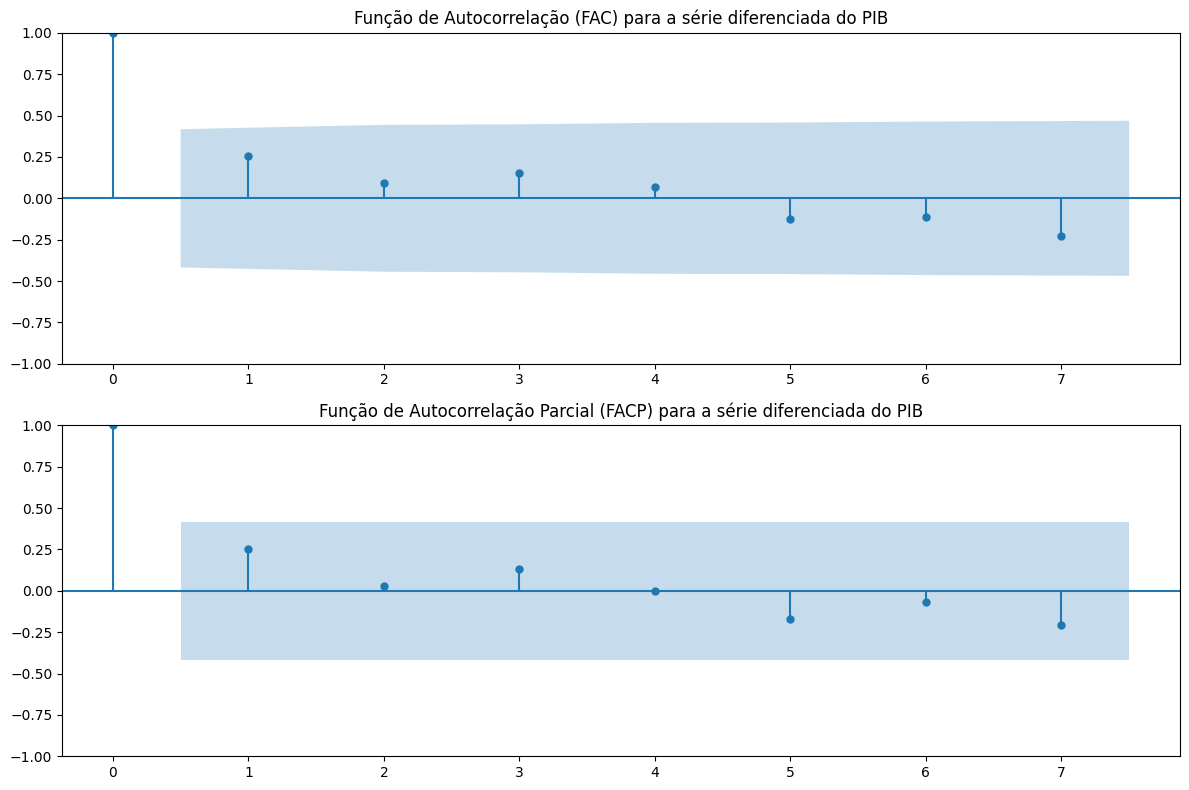
\includegraphics[width=1.0\textwidth]{images/FAC_FACP_ARIMA.png}
	
	\vspace{5pt} % Espaçamento sutil entre a imagem e a fonte
	\centering
	\small Fonte: Elaborado pelo autor (2026).
\end{figure}

Porém na imagem, parece não haver uma quebra significativa, na realidade ambos os teste se assemelham a um ruído branco. O mesmo comportamento pode ser verificado na tabela \ref{}. Porém apesar dos teste \ac{fac} e \ac{facp} serem úteis para estimação eles não são determinantes dos parâmetros. Para além disso o ARIMA apresenta sua vantagem de ser uma modelo leve, podemos testar várias combinações de ARIMA, com valores variados de p e q, e verificar o que se sai melhor.

Para encontrar o melhor modelo nesse momento utilizamos os critérios de O AIC (Critério de Informação de Akaike) e o BIC (Critério de Informação Bayesiano). E com base em ambos o modelo ARIMA(1,1,1) foi o modelo que obteve o melhor desempenho. O melhores modelos podem ser verificados na tabela \ref{}. Mas além do modelo e sair bem, uma boa prática é testar seus resíduos, utilizaremos para isso os testes Ljung-Box para verificar autocorrelação dos resíduos, e Jarque-Bera para verificar normalidade dos resíduos.


% Montar a tabela depois, estou com deveras preguiça nesse momento
Ljung-Box:
lb_stat  lb_pvalue
1  0.021001   0.884775
2  0.027370   0.986408
3  0.028403   0.998738
4  0.028621   0.999899
5  0.042300   0.999981

Jarque-Bera:
Estatística: 336.5530
p-valor:     0.0000
Assimetria:  4.2367
Curtose:     19.7149

A partir dos resultados de Ljung-Box, não há evidências estatísticas de autocorrelação nos resíduos até o lag 5. E Pelo estatística Jarque-Bera não há evidências estatísticas suficientes para rejeitar a hipótese de normalidade dos resíduos ao nível de 5\%. Ou seja o modelo ARIMA(1,1,1) parece ser um ótimo candidato. Na tabela \ref{} podemos ver o resumo do modelo.

% Vou resolver tenha paciência
                               SARIMAX Results                                
==============================================================================
Dep. Variable:               PIB Real   No. Observations:                   23
Model:                 ARIMA(1, 1, 1)   Log Likelihood                -259.175
Date:                Thu, 01 Oct 2026   AIC                            524.351
Time:                        00:00:36   BIC                            527.624
Sample:                             0   HQIC                           525.122
- 23                                         
Covariance Type:                  opg                                         
==============================================================================
coef    std err          z      P>|z|      [0.025      0.975]
------------------------------------------------------------------------------
ar.L1          0.9541      0.060     15.840      0.000       0.836       1.072
ma.L1         -0.9210      0.086    -10.720      0.000      -1.089      -0.753
sigma2      1.197e+09   8.11e-12   1.47e+20      0.000     1.2e+09     1.2e+09
===================================================================================
Ljung-Box (L1) (Q):                   0.88   Jarque-Bera (JB):                 1.52
Prob(Q):                              0.35   Prob(JB):                         0.47
Heteroskedasticity (H):               2.31   Skew:                            -0.62
Prob(H) (two-sided):                  0.29   Kurtosis:                         2.66
===================================================================================


Porém esse modelo ainda tem alguns problemas. O modelo tem apenas 23 observações, isso reduz a confiabilidade do modelo, porém isso é uma realidade econômica e das agências de coleta de dados que não tem séries contínuas em décadas\footnote{teremos um problema muito grande com isso em uma série específica, mas trataremos disso posteriormente}. 
O AR calculado é muito próximo de 1, isso implica que o fator autoregressivo é muito persistente, em uma série como o PIB isso significa um choque ocorrido hoje tende a continuar influenciando a série por vários períodos. Mas por outro lado o MA quase anula o AR, ou seja, o fator MA ser -0.9210, está praticamente anulando o AR: 0.9541, os choques tem um efeito contrário muito forte. Esse cancelamento de fatores leva uma matriz de covariância quase singular, indicando uma forte relação dos dois fatores.

Esses problemas são reais, mas falam mais da natureza da série do que propriamente de uma falha do ARIMA, estamos falando de uma série anual do PIB que é uma frequência baixa, optamos por trunca-la para ter uma parcimônia entre modelos no sentido tamanho da série. E mesmo assim encontramos um modelo relativamente bom, inclusive capturando um comportamento típico do PIB brasileiro. Existe uma forte tendência de manter o comportamento das séries anteriores apontado pelo AR, isso é explicado pelas tendências de crescimento e queda que existiram durante o período analisado, mas para além disso o MA tem um força puxando para equalizar, ou seja a tendência inercial é anulada por fator de média móvel. Veremos na série temporal isso mais de perto.

Mas antes precisamos ver realmente essa série, falamos do modelo de sua aplicação, mas ainda não apresentamos a série, porém agora podemos olhar a série não simplesmente como um gráfico de linha do PIB, mas sim como uma economia real e a interpretação econométrica sobre essa série.




